\part{Systems of linear equations I - Iterative methods}
\section{Introduction}
\subsection*{General}
\begin{frame}[label=contents_lin3]
  \frametitle{Today's outline}
  \mode<beamer>{
    \only<1>{\tableofcontents}
  }
  \only<2>{\tableofcontents[currentsection,currentsubsection]}
\end{frame}

\section{Sparse matrices}
\subsection*{Sparse matrices}

\begin{frame}[fragile]
  \frametitle{Sparse matrices}
  \begin{itemize}
    \item In many engineering cases, we deal with sparse matrices (as opposed to dense matrices)
    \item A matrix is sparse when it mostly consists of zeros
    \item Linear systems where equations depend on a limited number of variables (e.g. spatial discretization)
    \item Storing zeros is not very efficient:
    \begin{lstlisting}
# sparse_system_size.py
import sys
import numpy as np
import scipy.sparse as sparse
N = 10000
full_identity_matrix = np.eye(N)
full_size_in_memory = sys.getsizeof(full_identity_matrix)
sparse_identity_matrix = sparse.eye(N)
sparse_size_in_memory = sys.getsizeof(sparse_identity_matrix)
print(f'Full: {full_size_in_memory/1024**2} MB; sparse: {sparse_size_in_memory} b.')
    \end{lstlisting}
    \item Sparse matrix formats: e.g. Yale, CRS, CSC
\end{itemize}
\end{frame}

\begin{frame}[fragile]
  \frametitle{Sparse matrix storage format}
  \begin{columns}
  \column{0.6\textwidth}
  \begin{itemize}
    \item Example: Yale storage format, storing 3 vectors:
    \begin{itemize}
      \item \lstinline$A = np.array([5 8 3 6])$
      \item \lstinline$IA = np.array([0 1 2 3 4])$
      \item \lstinline$JA = np.array([0 1 2 1])$
    \end{itemize}
  \end{itemize}
  \column{0.4\textwidth}
  \[
   A = 
   \begin{bmatrix}
    5 & 0 & 0 & 0\\
    0 & 8 & 0 & 0\\
    0 & 0 & 3 & 0\\
    0 & 6 & 0 & 0
    \end{bmatrix}
  \]
  \end{columns}
  \begin{itemize}
    \item \lstinline$A$ stores the non-zero values
    \item \lstinline$IA$ stores the index in A of the first non-zero in row i
    \item \lstinline$JA$ stores the column index
    \item Note: zero-based indices are used here!
\end{itemize}
\end{frame}

\begin{frame}[fragile]
  \frametitle{Sparse matrix layout examples}
  \begin{center}
   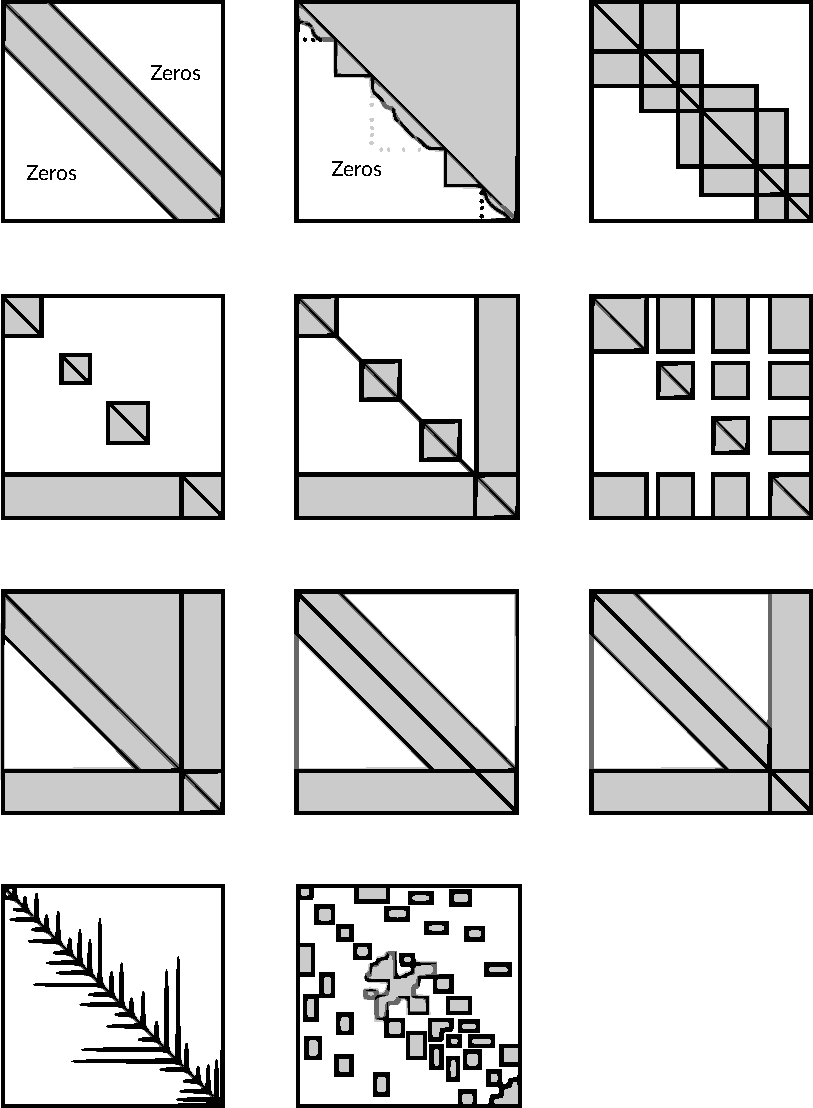
\includegraphics[height=0.8\textheight]{sparse-overview}
  \end{center}
\end{frame}

\section{Laplace's equation}
\subsection*{Laplace's equation}
\againframe<2>{contents_lin3}
\begin{frame}[fragile]
  \frametitle{Laplace's equation}
  \begin{columns}
  \column{0.7\textwidth}
  \begin{align*}
    \frac{\partial T}{\partial t} &= \alpha \nabla^2 T \\
    T &= \text{Temperature} \\
    \alpha &= \text{Thermal diffusivity}
  \end{align*}
  \pause
  \begin{center}
      \begin{tikzpicture}[scale=0.4]
      \draw[black,thick,->] (-0.3,-0.3)-- node[at end,anchor=north]{$x$}(7,-0.3);
      \draw[black,thick,->] (-0.3,-0.3)-- node[at end,anchor=east]{$y$} (-0.3,7);
      \draw[thick,draw=tuelblue,fill=tuegreen] (0,0) rectangle +(6,6);
      \node[anchor=west] at (6,3) {$T=T_{b4}$};
      \node[above,anchor=south] at (3,6.5) {$T=T_{b2}$};
      \node[below,anchor=north] at (3,-0.5  ) {$T=T_{b1}$};
      \node[left of=3pt] at (0,3) {$T=T_{b3}$};
%       \node at (0.3,0.3) (A) {};
%       \node at (0.3,5.7) (B) {};
%       \node at (5.7,5.7) (C) {};
%       \node at (5.7,0.3) (D) {};
%       \draw[thick,tuered] (A) -- node[midway,anchor=east] {$T=T_{b3}$} (B);
%       \draw[thick,tuegreen] (B) -- node[midway,anchor=south] {$T=T_{b2}$} (C);
%       \draw[thick,tueorange] (C) -- node[midway,anchor=east] {$T=T_{b4}$} (D);
%       \draw[thick,tuepurple] (D) -- node[midway,anchor=south] {$T=T_{b1}$} (A);
      \end{tikzpicture}
    \end{center}
    \pause
  \column{0.3\textwidth}
  In steady state:
  \[
   \nabla^2 T = 0
  \]
  \vskip2em
  \[
   \frac{\partial^2T}{\partial x^2} + \frac{\partial^2T}{\partial y^2} = 0
  \]
\end{columns}
\end{frame}

\begin{frame}[fragile]
  \frametitle{Discretization of Laplace's equation (I)}
  \begin{columns}
  \column{0.6\textwidth}
%     \vskip-2em
    \hspace*{-2em}
    \begin{tikzpicture}[scale=0.75,font=\sffamily\scriptsize]
      \foreach \x in {0,...,5}
        \foreach \y in {0,...,5} 
          {
    %        \pgfmathtruncatemacro{\label}{\x - 5 *  \y +21}
          \ifthenelse{\x=0 \OR \x=5 \OR \y=0 \OR \y=5}{\node [gdot,fill=tuered]  (\x\y) at (1.5*\x,1.5*\y) {};}
          \node [gdot,fill=tueblue]  (\x\y) at (1.5*\x,1.5*\y) {};} 

        \foreach \x [count=\xi] in {0,...,4}
          \foreach \y [count=\yi] in {0,...,4}  
            \draw (\x\y)--(\x\yi)-- (\xi\yi)--(\xi\y)--(\x\y);% (\y\x)--(\yi\x) ;
        
        \onslide<2->{
	  \node[anchor=east] at (00.west) {$j=1$};
	  \node[anchor=east] at (01.west) {$j=2$};
	  \node[anchor=east] at (02.west) {$j=3$};
	  \node[anchor=east] at (04.west) {$j=N_y-1$};
	  \node[anchor=east] at (05.west) {$j=N_y$};
	  \node[anchor=north] at (00.south) {$i=1$};
	  \node[anchor=north] at (10.south) {$i=2$};
	  \node[anchor=north] at (20.south) {$i=3$};
	  \node[anchor=north] at (40.south) {$i=N_x-1$};
	  \node[anchor=north west] at (50.south) {$i=N_x$};
	}
	
	\onslide<3->{
	  \node[anchor=south west] at (00.north east) {$T_1$};
	  \node[anchor=south west] at (10.north east) {$T_2$};
	  \node[anchor=south west] at (20.north east) {$T_3$};
	  \node[anchor=south west] at (30.north east) {$T_4$};
	  \node[anchor=south west] at (40.north east) {$T_5$};
	  \node[anchor=south west] at (50.north east) {$T_6$};
	  \node[anchor=south west] at (01.north east) {$T_{N_x+1}$};
	  \node[anchor=south west] at (11.north east) {$T_{N_x+2}$};
	  \node[anchor=south west] at (21.north east) {$T_{N_x+3}$};
	  \node[anchor=south west] at (51.north east) {$T_{2N_x}$};
	  \node[anchor=south]      at (55.north) {$T_{(N_y-1)N_x+1}$};
	}
      \end{tikzpicture}
%     \end{center}
  \hfill
  \column{0.35\textwidth}
  \begin{itemize}
    \item<1-> Define a grid of points in $x$ and $y$
    \item<2-> Index of the grid points using 2D coordinates $i$ and $j$
    \item<3> Set up the equations using a 1D index system: $T_{i,j}=T_{i+N_x(j-1)}$
  \end{itemize}
  \end{columns}
\end{frame}

\begin{frame}[fragile]
  \frametitle{Discretization of Laplace's equation (II)}
  Estimate the second-order differentials: assume a piece-wise linear profile in the temperature: \vskip1em
  \begin{columns}
  \column{0.5\textwidth}
    \begin{tikzpicture}[scale=0.7,node distance=5mm]
      \draw[black,thick,->] (0,0)-- node[at end,anchor=north]{$x$}(7,0);
      \draw[black,thick,->] (0,0)-- node[at end,anchor=east ]{$T$}(0,5);
      \node [gdot,fill=tuered] (n1) at (1,0) {};
      \node [gdot,fill=tuered] (n2) at (3,0) {};
      \node [gdot,fill=tuered] (n3) at (5,0) {};
      \node [anchor=south,dot,color=black,fill=black] (e1) at (1,1) {};
      \node [anchor=south,dot,color=black,fill=black] (e2) at (3,2) {};
      \node [anchor=south,dot,color=black,fill=black] (e3) at (5,4) {};
      \node [below=1mm of e1.center,anchor=north west] (e4) {$T_{i-1}$};
      \node [below=1mm of e2.center, anchor=north west] (e5) {$T_{i}$};
      \node [below=1mm of e3.center,anchor=north west] (e6) {$T_{i+1}$};
      \draw[black,thick] (e1.center) -- (e2.center) -- (e3.center);
      \draw[black,thick,<->] (1,-0.5) -- node[midway, below] {$\Delta x$} (2.9,-0.5);
      \draw[black,thick,<->] (3.1,-0.5) -- node[midway, below] {$\Delta x$} (5,-0.5);
      \end{tikzpicture}
%     \end{center}
  \hfill
  \column{0.35\textwidth}
  \pause
  \begin{align*}
    \frac{\partial^2T}{\partial x^2} \approx \frac{\left.\frac{\partial T}{\partial x}\right|_{i+\frac{1}{2}}-\left.\frac{\partial T}{\partial x}\right|_{i-\frac{1}{2}}}{\Delta x} \\[15pt]
    \approx \frac{ \frac{\left(T_{i+1,j}-T_{i,j}\right)}{\Delta x} - \frac{\left(T_{i,j}-T_{i-1,j}\right)}{\Delta x}}{\Delta x}\\[15pt]
    = \frac{T_{i+1,j}-2T_{i,j}+T_{i-1,j}}{(\Delta x)^2}
  \end{align*}
  \end{columns}
\end{frame}

\begin{frame}[fragile]
  \frametitle{Discretization of Laplace's equation (III)}
  The $y$-direction is derived analogously, so that the 2D Laplace's equation is discretized as:
  \[
    \frac{T_{i+1,j}-2T_{i,j}+T_{i-1,j}}{(\Delta x)^2} + \frac{T_{i,j+1}-2T_{i,j}+T_{i,j-1}}{(\Delta y)^2} = 0
  \]
  \pause
  Use a single index counter ${k=i+N_x(j-1)}$, so that the equation becomes:
  \[
    \frac{T_{k+1}-2T_k+T_{k-1}}{(\Delta x)^2} + \frac{T_{k+N_x}-2T_k+T_{k-N_x}}{(\Delta y)^2} = 0
  \]
  \pause
  For an equal spaced grid $\Delta x = \Delta y = 1$:
  \tikz{\node[emphblock, text width=\textwidth,]{\[
   T_{k-N_x} + T_{k-1} - 4T_k + T_{k+1} + T_{k+N_x} = 0
   \]
   \[
      \Rightarrow AT=b
   \]\vskip1ex
   %\Rightarrow T_k = \frac{T_{k-N_x} + T_{k-1} + T_{k+1} + T_{k+N_x}}{4}
  };}
\end{frame}

\section{Creating a sparse system}
\subsection*{A sparse matrix}
\againframe<2>{contents_lin3}
\begin{frame}[fragile]
  \frametitle{Creating the linear system}
  \vskip-1em
  \[
   T_{k-N_x} + T_{k-1} - 4T_k + T_{k+1} + T_{k+N_x} = 0
  \]
  Create a \emph{banded} matrix $A$: the main diagonal $k$ contains -4, whereas the bands at $k-1$, $k+1$, $k-N_x$ and $k+N_x$ contain a 1. Boundary cells just contain a 1 on the main diagonal so that the temperature is equal to $T_b$ (e.g. $T_1 = 1T_b$).\\
  \vskip1em
  \hspace*{8em}
  ${
    \begin{bmatrix}
      1 & 0 & 0 & 0 & 0 & 0 & 0 & 0 & \cdots & 0\\
      0 & 1 & 0 & 0 & 0 & 0 & 0 & 0 & \cdots & 0\\
    \vdots & \vdots & \vdots & \vdots & \vdots & \vdots & \vdots & \vdots & \ddots & \vdots\\
     \cdots & 1 & \cdots & 1 & -4 & 1 &\cdots & 1 & \ddots & 0\\
     0 & \cdots & 1 & \cdots & 1 & -4 & 1 &\cdots & 1 & \vdots\\
     \vdots & \vdots & \vdots & \vdots & \vdots & \vdots & \vdots & \vdots & \ddots & \vdots\\
     0 & 0 & 0 & 0 & 0 & 0 & 0 & 0 & 1 & 0\\
     0 & 0 & 0 & 0 & 0 & 0 & 0 & 0 & 0 & 1\\
    \end{bmatrix}
    \begin{bmatrix}
    T_1\\
    T_2\\
    \vdots\\
    T_k\\
    T_k+1\\
    \vdots\\
    T_{(N_y-1)N_x}\\
    T_{(N_y-1)N_x+1}
   \end{bmatrix} = 
   \begin{bmatrix}
    T_b\\
    T_b\\
    \vdots\\
    0\\
    0\\
    \vdots\\
    T_b\\
    T_b
   \end{bmatrix}}$
\end{frame}

\begin{frame}[fragile]
  \frametitle{Creating the linear system}
  \vskip-3em
  \[
   T_{k-N_x} + T_{k-1} - 4T_k + T_{k+1} + T_{k+N_x} = 0
  \]
  Create a \emph{banded} matrix $A$ by setting the coefficients for the internal cells:
  \begin{lstlisting}
# create_sparse_system.py
import numpy as np
import scipy.sparse as sps

Nx = 5 # Number of points along x direction
Ny = 5 # Number of points in the y direction
Nc = Nx*Ny # Total number of points
A = sps.diags([1,1,-4,1,1],[-Nx,-1,0,1,Nx],shape=(Nc,Nc))
A = sps.csr_matrix(A)
b = np.zeros([Nc,1])
  \end{lstlisting}
  The function \lstinline$sps.diags$ uses the following arguments:
  \begin{itemize}
   \item The coefficients that have to be put on the diagonals
   \item The position of the bands with respect to the main diagonal
   \item Size of the resulting matrix (in our case square $N_xN_y \times N_xN_y$)
  \end{itemize}
\end{frame}

\begin{frame}[fragile]
  \frametitle{Matrix sparsity}
  \begin{columns}
  \column{0.5\textwidth}
  
  \begin{itemize}
   \item Let's check the matrix layout:
   \begin{lstlisting}
import matplotlib.pyplot as plt
# ... (generate banded matrix) ... 
plt.spy(A)
plt.show()
   \end{lstlisting}
    \item This command shows the non-zero values of a matrix
    \item Apart from the main diagonal, there are offset bands!
  \end{itemize}
  \column{0.5\textwidth}
    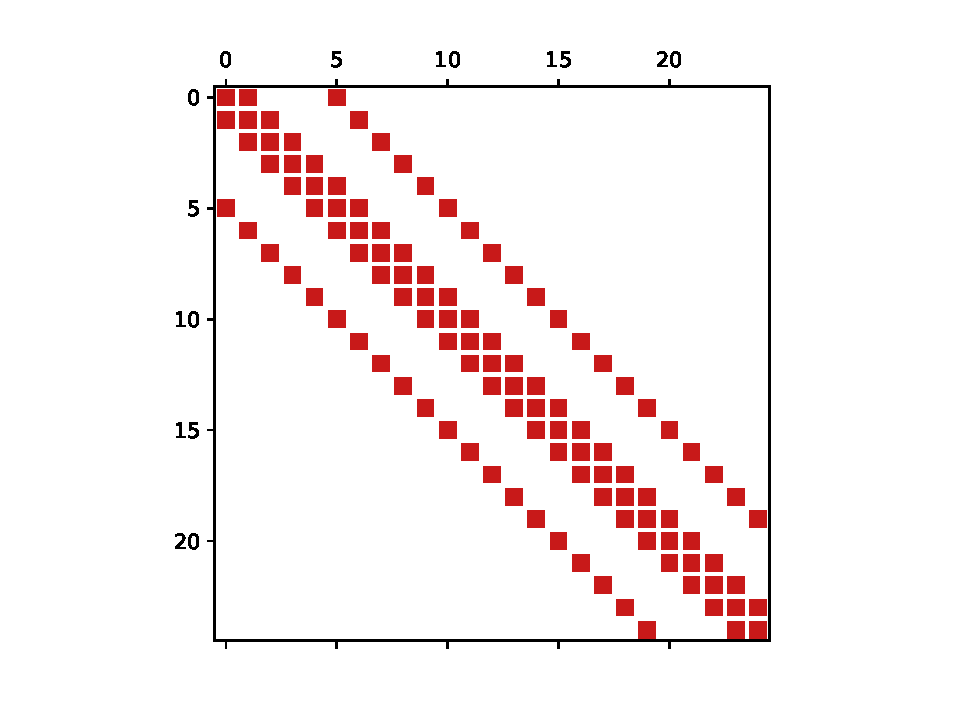
\includegraphics[width=\columnwidth]{mplspy}
  \end{columns}
\end{frame}

\subsection*{Boundary conditions}
\begin{frame}[fragile]
  \frametitle{About boundary conditions}
  \begin{itemize}
    \item For the nodes on the boundary, we have a simple equation:
    \[
      T_{k,\text{boundary}} = \text{Some fixed value}
      \]
      \item However, we have set all nodes to be a function of their neighbors...
      \item Find the boundary node indices using $k = i + j\times Nx$ %$k = i + Nx(j-1)$
      \begin{itemize}
        \item $i = 0$, $j = 0\rightarrow Ny-1$
        \item $i = Nx-1$, $j = 0\rightarrow Ny-1$
        \item $j = 0$, $i = 0\rightarrow Nx-1$
        \item $j = Ny-1$, $i = 1\rightarrow Nx-1$
      \end{itemize}
      \item Reset the row in $A$ to zeros, set $A_{kk}$ = 1
      \item Set value in rhs: $b_k = T_{k,\text{boundary}}$
      \item Boundary conditions are often more elaborate to implement!
  \end{itemize}
\end{frame}
  
\begin{frame}[fragile]
  \frametitle{Partial implementation of the boundary conditions}
  See \lstinline$extend_sparse_system.py$.
  \begin{lstlisting}[]
def get_boundary_condition_indices(Nx,Ny):
    idxS = np.arange(0,Nx)    # Bottom row
    idxN = (Ny-1)*(Nx)+idxS   # Top row
    idxW = np.arange(Ny)*(Nx) # Left column
    idxE = idxW+(Nx-1)        # Right column
    boundary_cells = {"south": idxS, "north": idxN, 'west': idxW, 'east': idxE,
    'total': np.unique(np.concatenate((idxS,idxW,idxE,idxN)))}
    return boundary_cells

def set_boundary_conditions(A,b,Tb,Nx,Ny):
    bc_idx = get_boundary_condition_indices(Nx,Ny)

    # For all the boundary cells:
    A[bc_idx['total'],:] = 0 # Reset matrix coefficients in row
    A[bc_idx['total'],bc_idx['total']] = 1 # Add a 1 on the main diagonal
    # Set temperature for each side separately
    b[bc_idx['north']] = Tb['N']
    b[bc_idx['south']] = Tb['S']
    b[bc_idx['east']] = Tb['E']
    b[bc_idx['west']] = Tb['W']
    
    return A,b 
  \end{lstlisting}
\end{frame}

\begin{frame}[fragile]
  \frametitle{How applying boundary conditions affects the linear system}
  \begin{columns}
    \column{0.5\textwidth}
      \begin{itemize}
        \item Create a dictionary that holds the temperature at each boundary:
        \begin{lstlisting}
Tb = {'N': 10, 'S': 20, 'E': 30, 'W': 40}
        \end{lstlisting}
        \item Call the function and (note that A and b are changed because they are passed by reference):
        \begin{lstlisting}
set_boundary_conditions(A,b, Tb, Nx, Ny)
        \end{lstlisting}
        \item Check the new structure of the matrix and the right hand side:
        \begin{lstlisting}
f, (ax1,ax2) = plt.subplots(1, 2,sharey='all')
ax1.spy(A)
ax2.spy(sps.csr_array(b))
plt.show()
        \end{lstlisting}
      \end{itemize}
    \column{0.5\textwidth}
      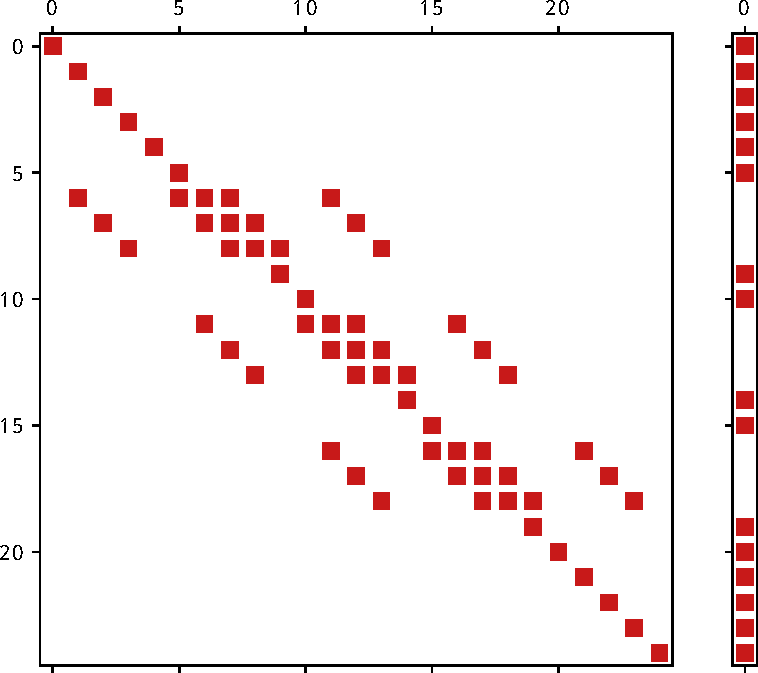
\includegraphics[width=\columnwidth]{figures/spab.pdf}
  \end{columns}
\end{frame}

\subsection*{Solving the equation}
\begin{frame}[fragile]
  \frametitle{A full program, including solver}
  \begin{lstlisting}[linewidth=1.05\textwidth]
    # Setup
    Nx, Ny = 50, 50 # Number of points along x, y direction
    Tb = {'N': 10, 'S': 20, 'E': 30, 'W': 40}
    
    # Create linear system
    Nc = Nx*Ny # Total number of points
    A = sps.diags([1,1,-4,1,1],[-Nx,-1,0,1,Nx],shape=(Nc,Nc))
    A = sps.csr_matrix(A)
    b = np.zeros([Nc,1])
    set_boundary_conditions(A,b, Tb, Nx, Ny)
    
    # Solve
    T_solution = sps.linalg.spsolve(A,b)
    
    # Postprocessing
    x,y = np.meshgrid(range(Nx), range(Ny))
    fig, ax = plt.subplots(1,1,subplot_kw=dict(projection='3d'))
    surf = ax.plot_surface(x,y,T_solution.reshape(Nx,Ny),cmap=cm.inferno,linewidth=0.1,edgecolor='black')
    fig.colorbar(surf, shrink=0.5, aspect=5,label='Temperature [$^\circ$C]')
    ax.set(xlabel='X [a.u.]', ylabel='Y [a.u.]', zlabel='T [$^\circ$C]')
    plt.show()
  \end{lstlisting}
\end{frame}
  
\begin{frame}[fragile]
  \frametitle{Sample results}
  Solved for a $50\times50$ system with \lstinline$Tb = {'N': 10, 'S': 20, 'E': 30, 'W': 40}$
  \begin{center}
    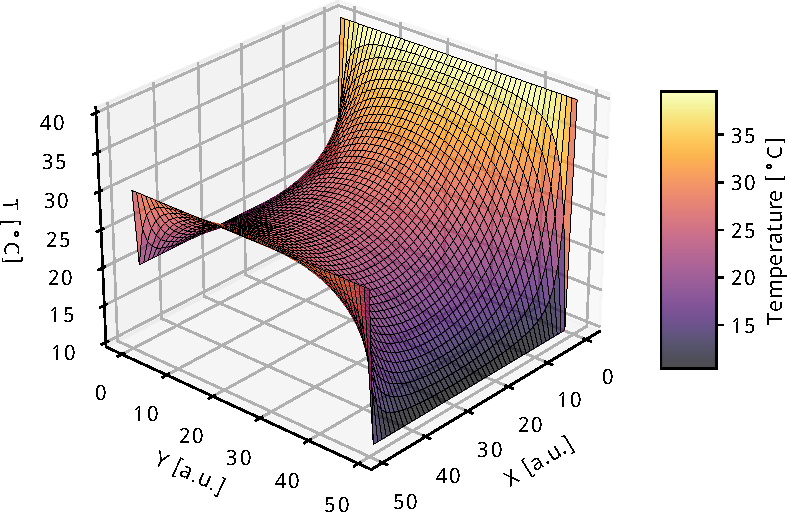
\includegraphics[width=0.7\textwidth]{laplace_py_50x50}
  \end{center}
\end{frame}

{\nologo
\begin{frame}[fragile]
  \frametitle{Exercise: Verify the numerical solution using Fourier-series}
  A Fourier-series expansion for the steady-state heat conduction in a flat plate is given for a domain: $x,y\in[0,1]$ , with fixed-temperature boundaries $T\big|_{x=0} = T\big|_{x=1} = T\big|_{y=0}=0$ and $T\big|_{y=1}=1$:
\[
    T = \frac{4}{\pi} \sum_{n=1}^\infty \frac{\sin\left(m \pi x \right)\sinh\left(m\pi y \right)}{m \sinh\left(m \pi \right)} \quad \text{with} \quad m=2n-1
\]
Compute and plot the exact temperature profile in the 2D plate, and compare it with the numerical solution:
  \begin{hints}
  Hints:
  \begin{itemize}
      \item Use meshgrid to create a mesh in $x$ and $y$
      \item Compute the temperature using the Fourier series, use vectorised computations over $x$ and $y$ so that only 1 loop (over n) is required.
      \item Solve the numerics for the same problem (note the boundary conditions)
      \item Compare the numerical and exact solutions (e.g. a plot).
  \end{itemize}
  \end{hints}
\end{frame}
}

\begin{frame}<beamer:1-|handout:0>[fragile]
  \frametitle{Exercise: Verify the numerical solution using Fourier-series}
    \begin{lstlisting}
% Generate the mesh
Nx, Ny = 25, 25
T_boundaries = {'N': 1, 'S': 0, 'E': 0, 'W': 0}
x,y = np.meshgrid(np.linspace(0,1,Nx),np.linspace(0,1,Ny))
T = np.zeros_like(x) (*@ \pause @*)
% Fourier series expansion
for n in range(1,50):
    m = 2*n-1
    T = T + (np.sin(m*np.pi*x) * np.sinh(m*np.pi*y)) / (m*np.sinh(m*np.pi))
T_exact = T*4/np.pi (*@ \pause @*)

# Compute numerical solution and difference
T_numerical = run_specific_case(Nx=Nx, Ny=Ny,Tb=T_boundaries).reshape(Nx,Ny)
T_diff = np.abs(T_numerical.reshape(Nx,Ny) - T_exact)

# Postprocessing (surface plot)
fig, (ax1,ax2,ax3) = plt.subplots(1,3,subplot_kw=dict(projection='3d'))
surf1 = ax1.plot_surface(x,y,T_numerical,cmap=cm.magma,linewidth=0.1,edgecolor='black', alpha=.7)
surf2 = ax2.plot_surface(x,y,T_exact,cmap=cm.magma,linewidth=0.1,edgecolor='black', alpha=.7)
surf3 = ax3.plot_surface(x,y,T_diff,cmap=cm.magma,linewidth=0.1,edgecolor='black', alpha=.7)

plt.show()
    \end{lstlisting}
\end{frame}


\begin{frame}[fragile]
  \frametitle{LU decomposition of a sparse matrix}
  \begin{columns}
  \column{0.35\textwidth}
    \begin{lstlisting}
# lu_spy_sparse.py
Nx, Ny = 5, 5
Nc = Nx*Ny
A = sps.diags([1,1,-4,1,1],[-Nx,-1,0,1,Nx],shape=(Nc,Nc))

P, L, U = spla.lu(A.todense()) (*@ \pause @*)

fig,(ax1,ax2) = plt.subplots(1,2)
ax1.spy(sps.lil_matrix(L))
ax1.set_title('LU Lower matrix')
ax2.spy(sps.lil_matrix(U))
ax2.set_title('LU Upper matrix')
plt.show()
    \end{lstlisting}
  \column{0.65\textwidth}
  \pause
  \begin{itemize}
    \item With LU decomposition we produce matrices that are less sparse than the original matrix.
    \item Sparse storage often required, and also numerical techniques that fully utilizes this!
  \end{itemize}\vskip2em
  
\includegraphics[width=0.9\columnwidth]{LU_spy}
  \end{columns}
\end{frame}
  
\begin{frame}[fragile]
  \frametitle{LU decomposition}
  \begin{itemize}
    \item LU decomposition and Gaussian elimination on a matrix like $A$ requires more memory (with 3D problems, the offset in the diagonal would even be bigger!)
    % \item In general extra memory allocation will not be a problem for MATLAB
    % \item MATLAB is clever, in that sense that it attempts to reorder equations, to move elements closer to the diagonal)
  \end{itemize} \pause
  Alternatives for elimination methods
  \begin{itemize}
    \item Use iterative methods when systems are large and sparse.
    \item Often such systems are encountered when we want to solve PDE’s of higher dimensions
  \end{itemize}
\end{frame}

\section{Iterative methods}
\subsection*{Introduction}
\againframe<2>{contents_lin3}

\begin{frame}[fragile]
  \frametitle{Examples of iterative methods}
  \begin{itemize}
    \item Jacobi method
    \item Gauss-Seidel method
    \item Succesive over relaxation \vskip2em
    \item \lstinline$scipy.sparse.bicg$ --- Bi-conjugate gradient method
    \item \lstinline$scipy.sparse.bicgstab$ --- Bi-conjugate gradient (stabilized) method
    \item \lstinline$scipy.sparse.cg$ --- Conjugate gradient method
    \item \lstinline$scipy.sparse.gmres$ --- Generalized minimum residuals method
\end{itemize}
\end{frame}

\subsection*{Jacobi method}
\begin{frame}[fragile]
  \frametitle{The Jacobi method}
  \begin{itemize}
     \item In our example we derived the following equation:
    \[
     T_{k-N_x} + T_{k-1} - 4T_k + T_{k+1} + T_{k+N_x} = 0
    \]
    \item Rearranging gives:
    \[
      T_k = \frac{T_{k-N_x} + T_{k-1} + T_{k+1} + T_{k+N_x}}{4}
    \]\pause
    \item In the Jacobi scheme the iteration proceeds as follows:
    \begin{enumerate}
      \setlength{\itemindent}{1cm}
      \item Start with an initial guess for the values of $T$ at each node\pause
      \item Compute updated values and store a new vector:
        \[
          T_k^\text{new} = \frac{T_{k-N_x}^\text{old} + T_{k-1}^\text{old} + T_{k+1}^\text{old} + T_{k+N_x}^\text{old}}{4}
        \]\pause
      \item Do this for all nodes\pause
      \item Repeat the procedure until converged
    \end{enumerate}
  \end{itemize}
\end{frame}

\begin{frame}[fragile]
  \frametitle{Jacobi method for Laplace's equation}
  \vskip-1em
  \begin{columns}
    \column{0.6\textwidth}
    \begin{lstlisting}[basicstyle=\scriptsize\ttfamily]
  # Grid size
  Nx,Ny = 40,40 (*@ \pause @*)
  # The temperature field + boundaries
  T = np.zeros([Nx,Ny])
  T[0,:] = 40    # Left 
  T[Nx-1,:] = 60 # Right
  T[:,0] = 20    # Bottom
  T[:,Ny-1] = 30 # Top 
  Tnew = T.copy() (*@ \pause @*)
  
  T_stored = []
  store_it = [0,20,80,320] (*@ \pause @*)
  
  for iter in range(400):
      for i in range(1,Nx-1):
          for j in range(1,Ny-1): 
              Tnew[i,j] = (T[i-1,j]+T[i+1,j]+T[i,j-1]+T[i,j+1])/4
      T = Tnew

      if iter in store_it:
          T_stored.append(T.copy())
    \end{lstlisting}
    \vfill 
    \column{0.4\textwidth}
      \begin{lstlisting}[firstnumber=22]
# For plotting
x,y = np.meshgrid(range(Nx),range(Ny))
fig,axxs = plt.subplots(2,2,
    subplot_kw=dict(projection='3d'))
axxs.shape = (axxs.size)
for idx, ax in np.ndenumerate(axxs):
    ax.plot_surface(x,y,T_stored[idx[0]])
    ax.set_title(f'Iteration: {store_it[idx[0]]}')

plt.tight_layout()
plt.show()
      \end{lstlisting}
      \begin{itemize}
        \item Computation occurs on l. 17
        \item Use the copy() operator to store intermediate results
        \item Axes of multiple subplots are returned as \lstinline$np.array$, which we can iterate (l. 24+27)
      \end{itemize}
  \end{columns}
\end{frame}

\begin{frame}
  \frametitle{Laplace equation solved using Jacobi iterations}
  \begin{center}
    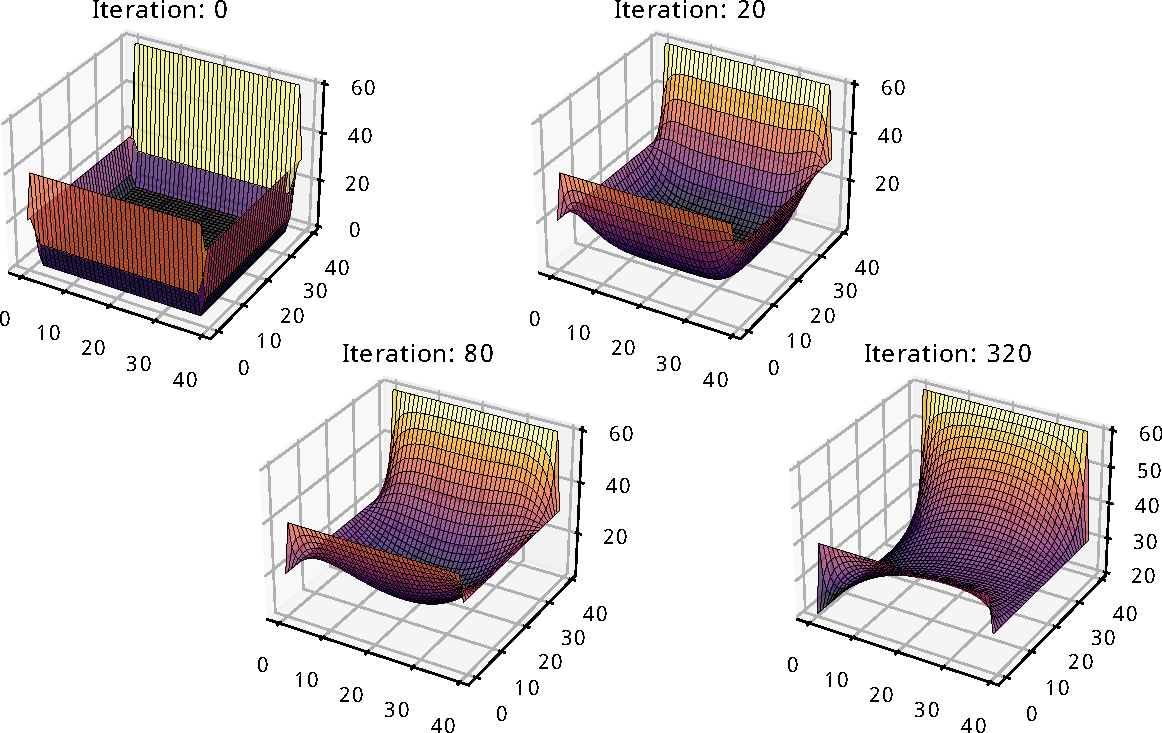
\includegraphics[width=0.8\textwidth]{figures/laplace_iter_jacobi.pdf}
  \end{center}
\end{frame}

\begin{frame}[fragile]
  \frametitle{About the straightforward implementation}
  \begin{itemize}
  
   \item The method as implemented works fine for a simple Laplace equation
%    \item We did not take into account the thermal diffusivity (set to unity)
%    \item We did not take into account the grid spacing (set to unity)
   \item For generic systems of linear equations, the implementation cannot be used.
  \end{itemize}\vskip2em\pause
 \tikz{\node[emphblock,text width=\textwidth]{We will now introduce the Jacobi method so it can be used for generic systems of linear equations.};}
\end{frame}

\begin{frame}[fragile]
  \frametitle{The Jacobi method with matrices}
  We can split our (banded) matrix $A$ into a diagonal matrix $D$ and a remainder $R$:\vskip1em
  \[
   A \quad =\quad  D \quad + \quad R
  \]
 \vskip2em
  \scalebox{0.6}{
  $
   \begin{bmatrix}
    \times & \times &  &  &  &  & \times &  & \\
    \times & \times & \times &   &   &   &   & \times &    \\
           & \times & \times & \times &   &   &   &   & \times \\
           &   & \times & \times & \times &   &   &   &   \\
      &   &   & \times & \times & \times &   &   &    \\
      &   &   &   & \times & \times & \times &   &   \\
      \times &   & &   &   & \times & \times & \times &   \\
      &   \times &   & &   &   & \times & \times & \times \\
      &   &   \times &   & &   &   & \times & \times \\
   \end{bmatrix} = 
   \begin{bmatrix}
    \times &  &  &  &  &  &  &  & \\
     & \times &  &   &   &   &   &  &    \\
           &  & \times &  &   &   &   &   &  \\
           &   &  & \times &  &   &   &   &   \\
     &   &   &  & \times &  &   &   &    \\
      &  &   &   &  & \times &  &   &   \\
      &   &  &   &   &  & \times &  &   \\
      &   &   &  &   &   &  & \times &  \\
      &   &   &   &  &   &   &  & \times \\
   \end{bmatrix} + 
   \begin{bmatrix}
     & \times &  &  &  &  & \times &  & \\
    \times &  & \times &   &   &   &   & \times &    \\
           & \times &  & \times &   &   &   &   & \times \\
           &   & \times &  & \times &   &   &   &   \\
      &   &   & \times &  & \times &   &   &    \\
      &   &   &   & \times &  & \times &   &   \\
      \times &   & &   &   & \times &  & \times &   \\
      &   \times &   & &   &   & \times &  & \times \\
      &   &   \times &   & &   &   & \times &  \\
   \end{bmatrix}$}
\end{frame}

\begin{frame}[fragile]
  \frametitle{Jacobi method: solving a system}
  \begin{itemize}
   \item We can solve $AT=b$, now written generally as $Ax=b$, by:
   \begin{align*}
      Ax&=b\\
     (D+R)x &= b \\
      Dx &= b -Rx \\
      Dx^\text{new} &= b - Rx^\text{old} \\
       x^\text{new} &= D^{-1}(b-Rx^\text{old})
   \end{align*}
   \item Using the $n$ and $n+1$ notation for old and new time steps, we find in general:
   \[
    x^{n+1} = D^{-1}\left(  b-Rx^n\right)
   \]
   \[
    x_i^{n+1} = \frac{1}{A_{ii}}\left(b_i - \sum_{j\neq i} A_{ij}x_j^n\right)
   \]
  \end{itemize}
\end{frame}

\begin{frame}[fragile]
  \frametitle{Diagram of the Jacobi method}
  \begin{tikzpicture}[scale=0.5,font=\tiny,node distance = 25pt, auto,->=stealth,point/.style={circle,fill=red,minimum size=0pt,inner sep=0pt}]
    \tikzstyle{block2} = [rectangle,minimum height=1em,draw=maincolor,fill=maincolor!20,text centered,rounded corners,minimum height=2em,thick,text width=1.5cm]
    \node[block2]                 (start) {Set $T^\text{old}$ = a guess};
    \node[block2, right=of start,visible on=<2->] (calc)  {Calculate the new node solution with previous values.};
    \node[block2, right=of calc,visible on=<3->] (check1) {Have all nodes been updated?};
    \node[block2, right=of check1,,visible on=<5->,text width=2cm] (tol) {Tolerance check: $\frac{\mynorm{x^{n+1}-x^n}}{\mynorm{x^n}} \leq \text{tol} $?};
    \node[block2, above=of check1,visible on=<4->] (next) {Move to next node};
    \node[block2, above=of tol,visible on=<6->] (update) {Update $T^\text{old}=T^\text{new}$};
    \node[block2, below=of tol,visible on=<8->] (answer) {Report the answer as $T^\text{new}$};
    \draw[->,thick,black,visible on=<2->] (start.east) -- (calc.west);
    \draw[->,thick,black,visible on=<3->] (calc.east) -- (check1.west);
    \draw[->,thick,black,visible on=<5->] (check1.east) -- node[midway,above]{Yes} (tol.west);
    \draw[->,thick,black,visible on=<4->] (check1.north) -- node[midway]{No} (next.south);
    \draw[->,thick,black,visible on=<6->] (tol.north) -- node[midway,left] {No} (update.south);
    \draw[->,thick,black,visible on=<8->] (tol.south) -- node[midway,left] {Yes} (answer.north);
    \draw[->,thick,black,visible on=<7->] (update.north) |- ++(0,0.5cm) -| ($ (calc.north) + (-5mm,0)$);
    \draw[->,thick,black,visible on=<4->] (next.west) -| ($ (calc.north) + (5mm,0)$);
    
%     \draw[->,thick,black] (tol.north) -| ($ (digit.east) + (2mm,0) $) (calc.west);
%     \draw[->,thick,black] (start.east) -- (calc.west);
  \end{tikzpicture}
\end{frame}

\begin{frame}[fragile]
  \frametitle{The core of the solver}
  The solvers are shared in the library \lstinline$iterative_solvers.py$.
  \begin{lstlisting}[numbers=left]
# While not converged or max_it not reached
while xdiff >= tol and it_jac < max_it:
    x_old = x.copy()
    for i in range(N):
        s = 0
        for j in range(N):
            if not j == i:
                # Sum off-diagonal*x_old
                s = s+A[i,j] * x_old[j]
        # Compute new x value
        x[i] = (b[i]-s)/A[i,i]

    # Increase number of iterations
    it_jac = it_jac+1;
    xdiff = np.linalg.norm((x-x_old))/np.linalg.norm(x)

return x,it_jac
  \end{lstlisting}
  \pause
  Try to call it for the Laplace equation, instead of using \lstinline$spla.linalg.solve$.
\end{frame}

\begin{frame}[fragile]
  \frametitle{A few details on this algorithm}
  \begin{itemize}
   \item The while loop holds two aspects
   \begin{itemize}
    \item A convergence criterion ($\frac{||(x-x_\mathrm{old}||}{||x||} \leq tol$). Some considerations are:
    \begin{itemize}
      \item $L_1$-norm (sum)
      \item $L_2$-norm (Euclidian distance)
      \item $L_\infty$-norm (max)
    \end{itemize}
    \item Protection against infinite loops (no convergence)
   \end{itemize}\pause
   \item Reset the sum for each row, before summing for the new unknown node
  \end{itemize}\pause
  \vskip1em
  \begin{itemize}
    \item Start vector x is not shown in the example, but should be there!
    \item It can have huge impact on performance!
    \item The for-loops also have a large performance penalty!
  \end{itemize}
\end{frame}

\begin{frame}[fragile]
  \frametitle{The solver using array indices}
  Make a copy of the Jacobian solver, and replace the for-loop by a vector-operation:
  \begin{lstlisting}[basicstyle=\scriptsize\ttfamily]
# While not converged or max_it not reached
while xdiff >= tol and it_jac < max_it:
    x_old = x.copy()
    for i in range(N):
        off_diag_idx = np.delete(np.arange(0,N),i)
        Aij_Xj = A[i,off_diag_idx]@x_old[off_diag_idx]

        # Compute new x value
        x[i] = (b[i]-Aij_Xj)/A[i,i]

    # Increase number of iterations
    it_jac = it_jac+1;
    xdiff = np.linalg.norm((x-x_old)/x);

return x,it_jac
\end{lstlisting}
\end{frame}

% \begin{frame}[fragile]
%   \frametitle{Iterations 1, 2, 3 and 10}
%   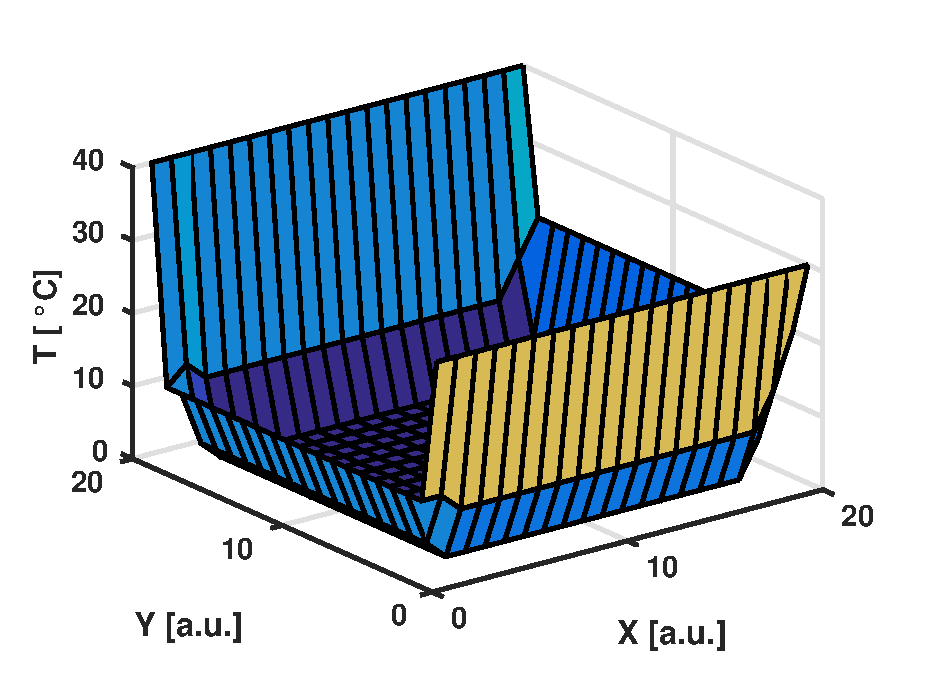
\includegraphics[width=0.35\textwidth]{it1} \hspace{0.5cm}
%   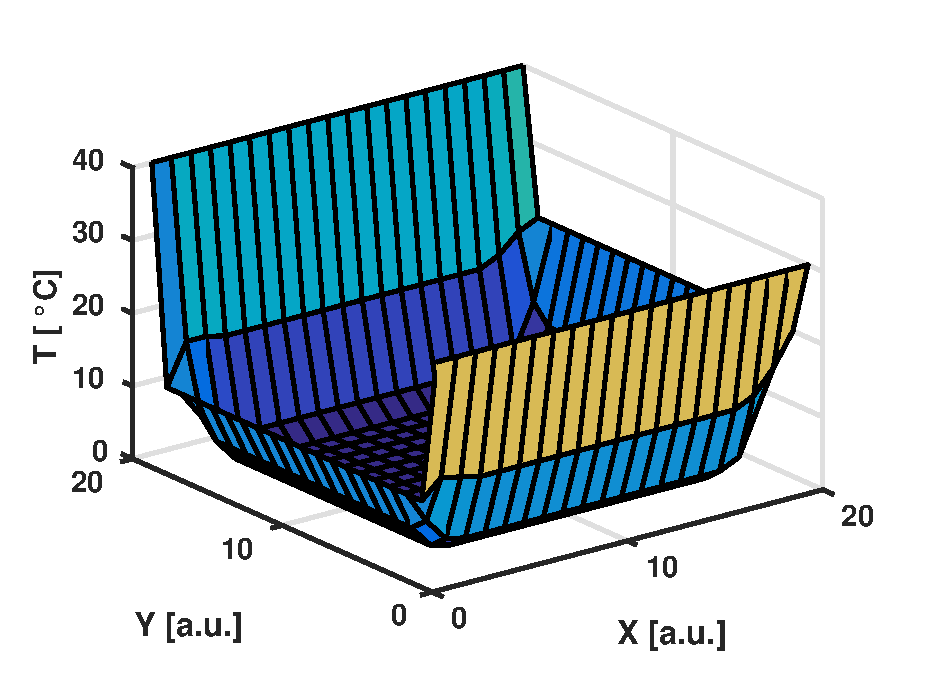
\includegraphics[width=0.35\textwidth]{it2}\\
%   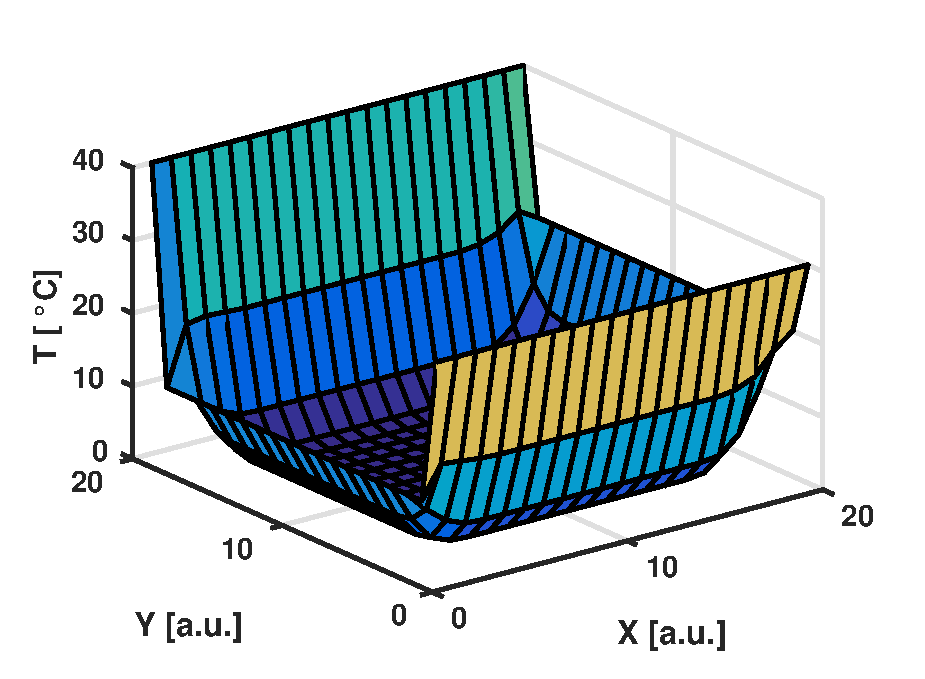
\includegraphics[width=0.35\textwidth]{it3} \hspace{0.5cm} 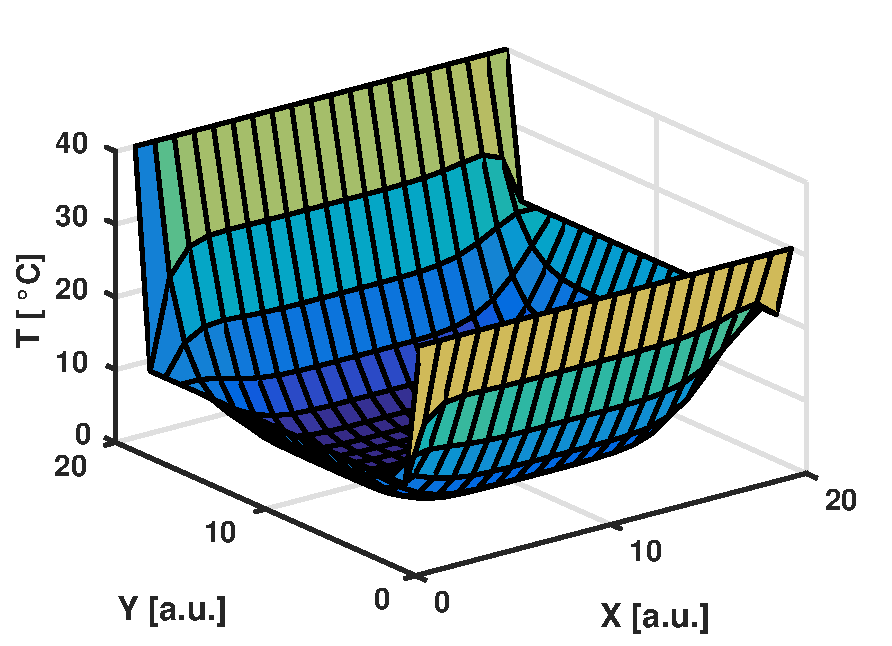
\includegraphics[width=0.35\textwidth]{it10}
% \end{frame}

\subsection*{Gauss-Seidel method}
\begin{frame}[fragile]
  \frametitle{Gauss-Seidel method}
  The Gauss-Seidel method is quite similar to Jacobi method
  \begin{itemize}
   \item The only difference is that the new estimate $x^\text{new}$ is returned to the solution $x^\text{old}$ as soon as it is completed
   \item For following nodes, the updated solution is used immediately \pause
   \item Our straightforward script (from the Jacobi method) is therefore changed easily:
   \begin{itemize}
    \item Do not create a \lstinline$Tnew$ array (save memory!)
    \item Do not store the solution in \lstinline$Tnew$, but simply in \lstinline$T$
    \item Do not perform the update step \lstinline$T=Tnew$
    \item See \lstinline$solve_laplace_gauss_seidel_basic.py$ for the algorithm.\pause
   \end{itemize}
   \item The straightforward script works well for the current Laplace equation, but we define the generic Gauss-Seidel algorithm on the following slides.
  \end{itemize}
\end{frame}

\begin{frame}[fragile]
  \frametitle{Gauss-Seidel method}
  \begin{itemize}
    \item Define a lower and strictly upper triangular matrix, such that $A = L + U$
    \item Now we can solve AT=b by:
    \begin{align*}
      (L+U)T &= b \\
      LT &= b - UT \\
      LT^\text{new} &= b - UT^\text{old} \\
      T^\text{new} &= L^{-1}(b-UT^\text{old})
   \end{align*}
     \item Using the $n$ and $n+1$ notation for old and new time steps, we find in for the general Gauss-Seidel method:
     \[
      x^{n+1} = L^{-1}\left(b-Ux^n\right)
     \]
     \[
      x_i^{n+1} = \frac{1}{A_{ii}}\left(b_i - \sum_{j<i} A_{ij}x_j^{n+1}- \sum_{j>i} A_{ij}x_j^n\right)
     \]
  \end{itemize}
\end{frame}

\begin{frame}[fragile]
  \frametitle{Implementation of the Gauss-Seidel method}
  The noteworthy differences with Jacobi are on lines 7--12:
  \begin{lstlisting}[basicstyle=\scriptsize\ttfamily]
# While not converged or max_it not reached
while xdiff >= tol and it_gs < max_it:
    x_old = x.copy()
    for i in range(N):
        s = 0
        for j in range(N):
            if j < i:
                # Sum off-diagonal*x
                s = s+A[i,j] * x[j]
            elif j > i:
                # Sum off-diagonal*x_old
                s = s+A[i,j] * x_old[j]

        # Compute new x value
        x[i] = (b[i]-s)/A[i,i]

    # Increase number of iterations
    it_gs = it_gs+1
    xdiff = np.linalg.norm((x-x_old))/np.linalg.norm(x)

return x,it_gs
\end{lstlisting}
\end{frame}

\section{Summary}
\subsection*{Summary}
\againframe<2>{contents_lin3}
\begin{frame}[fragile]
  \frametitle{Summary}
  \begin{itemize}
    \item Partial differential equations can be discretized into sparse systems of linear equations
    \item Sparse matrices can be stored in memory efficiently using specialised formats (e.g. compressed row storage)
    \item The Jacobi and Gauss–Seidel methods were introduced as iterative methods; other methods are based on the same principle (successive over-relaxation method, for example)
    \item Various implementation issues were discussed, e.g. vectorised computing, convergence tolerances
  \end{itemize}
\end{frame}

\begin{frame}[fragile]
  \frametitle{Direct methods vs. Iterative methods}
  \begin{itemize}
    \item Iterative methods converge \emph{gradually} to a solution while direct methods (possibly with partial pivoting) factorise a (set of) matrix(ces) which allow to compute the solution by \emph{substitution}.
    \item Direct methods generally use more memory, since they need to store also the result matrices.
    \item A strictly (or irreducibly) diagonally dominant matrix is a prerequisite for convergence of the Jacobi and Gauss-Seidel method.
    \item For real-life situations; 1D problems are generally solved with direct methods (LU decomposition). If you have systems of more than 1 dimension, a direct method still can be used, if there are no memory issues, otherwise an iterative method would be more attractive.
  \end{itemize}
\end{frame}

\section{Exercises}
\subsection*{Exercises}
\againframe<2>{contents_lin3}
\begin{frame}[fragile]
  \frametitle{Exercises}
  \begin{enumerate}
    \item Compute the computational complexity of the solvers discussed:
    \begin{itemize}
      \item Gauss-Jordan elimination and backsubstitution
      \item LU decomposition
      \item Jacobi
      \item Gauss-Seidel
    \end{itemize}
    \item Change the Gauss-Seidel solver function to its vectorized form and demonstrate the speed gains
    \item Implement the Successive over-relaxation method 
    \item Implement a Richardson iteration solver: 
      \[ x^{{(k+1)}}=x^{{(k)}}+\omega \left(b-Ax^{{(k)}}\right) \]
      with $\omega$ a scalar between 0 and 1.
  \end{enumerate}
\end{frame}